\documentclass[aspectratio=169,10pt]{beamer}
% Shared Beamer setup for Fall 2026 course slides.
\mode<presentation>{
  \usetheme{Madrid}
  \usecolortheme{default}
}

\definecolor{CalPolyGreen}{HTML}{154734}
\definecolor{CalPolyGold}{HTML}{BD8B13}
\definecolor{DeckInk}{HTML}{1F2933}
\definecolor{DeckMuted}{HTML}{5F6B7A}

\setbeamercolor{structure}{fg=CalPolyGreen}
\setbeamercolor{palette primary}{bg=CalPolyGreen,fg=white}
\setbeamercolor{palette secondary}{bg=DeckInk,fg=white}
\setbeamercolor{palette tertiary}{bg=CalPolyGold,fg=DeckInk}
\setbeamercolor{frametitle}{bg=CalPolyGreen,fg=white}
\setbeamercolor{title}{fg=CalPolyGreen}
\setbeamercolor{normal text}{fg=DeckInk,bg=white}
\setbeamercolor{block title}{bg=CalPolyGreen,fg=white}
\setbeamercolor{block body}{bg=black!3,fg=DeckInk}

\setbeamertemplate{navigation symbols}{}
\setbeamertemplate{footline}[frame number]
\setbeamertemplate{itemize item}{\color{CalPolyGold}$\blacktriangleright$}
\setbeamertemplate{itemize subitem}{\color{CalPolyGreen}$\bullet$}

\newcommand{\CourseNumber}{Course}
\newcommand{\CourseTitle}{Course Title}
\newcommand{\LectureNumber}{0}
\newcommand{\LectureTitle}{Lecture Title}
\newcommand{\LectureDate}{Date}
\newcommand{\CourseUnit}{Unit}

\newcommand{\coursenumber}[1]{\renewcommand{\CourseNumber}{#1}}
\newcommand{\coursetitle}[1]{\renewcommand{\CourseTitle}{#1}}
\newcommand{\lecturenumber}[1]{\renewcommand{\LectureNumber}{#1}}
\newcommand{\lecturetitle}[1]{\renewcommand{\LectureTitle}{#1}}
\newcommand{\lecturedate}[1]{\renewcommand{\LectureDate}{#1}}
\newcommand{\courseunit}[1]{\renewcommand{\CourseUnit}{#1}}

\author{Kirk Duran}
\institute{California Polytechnic State University, San Luis Obispo}
\date{\LectureDate}

\newcommand{\makedecktitle}{
  \begin{frame}[plain]
    \vspace{0.25in}
    {\usebeamerfont{title}\color{CalPolyGreen}\LectureTitle\par}
    \vspace{0.18in}
    {\large \CourseNumber{}: \CourseTitle\par}
    \vspace{0.08in}
    {\large Lecture \LectureNumber{} -- \LectureDate\par}
    \vfill
    {\small Kirk Duran \textbar{} Cal Poly, San Luis Obispo\par}
  \end{frame}
}

\newcommand{\placeholdernote}{
  \begin{block}{Placeholder}
    Replace these bullets with the final lecture material, examples, and in-class activities.
  \end{block}
}

\AtBeginSection[]{
  \begin{frame}{Roadmap}
    \tableofcontents[currentsection]
  \end{frame}
}

\graphicspath{{../assets/lecture-02/}}
\newcommand{\lectureimage}[2][1.75in]{\includegraphics[width=\linewidth,height=#1,keepaspectratio]{#2}}
\setbeamersize{text margin left=0.42in,text margin right=0.42in}

\coursenumber{CS 4880}
\coursetitle{Artificial Intelligence}
\lecturenumber{2}
\lecturetitle{Intelligent Agents}
\lecturedate{August 26, 2026}
\courseunit{1. Intelligent Agents}

\begin{document}

\makedecktitle

% ============================================================
% Opening: What do we mean by intelligence?
% ============================================================

\begin{frame}[shrink=20]{Intelligence: What Do We Want Out Of AI?}
  \begin{columns}[T,onlytextwidth]
    \begin{column}{0.48\textwidth}
      \begin{keyidea}
        Before we define an intelligent agent, we should ask what behavior we actually want from an AI system.
      \end{keyidea}
      \vspace{0.10in}
      \begin{enumerate}
        \item Be independent from constant human control.
        \item Solve problems rather than merely replay a fixed sequence.
        \item Be as good as us---or better---on the task we care about.
      \end{enumerate}
      \vspace{0.10in}
      \begin{activity}
        What do we mean by \emph{better}? Faster? Safer? More accurate? More adaptable? More human-like?
      \end{activity}
    \end{column}
    \begin{column}{0.47\textwidth}
      \lectureimage[2.0in]{goalsofai.png}
    \end{column}
  \end{columns}
\end{frame}

\begin{frame}{Self-Driving Cars}
  \begin{columns}[T,onlytextwidth]
    \begin{column}{0.52\textwidth}
      \begin{itemize}
        \item How does a self-driving car ``see'' the world?
        \item Is it following programmed rules, or adapting to new situations?
        \item How is this different from a simple remote-controlled car?
      \end{itemize}
      \vspace{0.16in}
      \begin{keyidea}
        The interesting part is not that the car moves. The interesting part is how it chooses what to do from what it perceives.
      \end{keyidea}
    \end{column}
    \begin{column}{0.42\textwidth}
      \lectureimage[2.0in]{selfdrivingcar.png}
    \end{column}
  \end{columns}
\end{frame}

\begin{frame}{Vacuum Bot}
  \begin{columns}[T,onlytextwidth]
    \begin{column}{0.52\textwidth}
      \begin{itemize}
        \item Your robot vacuum moves on its own, but is it thinking?
        \item How does it ``see'' the room?
        \item What kinds of choices does it make: straight-line movement, obstacle avoidance, room selection, charging?
        \item Is it following a preset routine, or does it adapt?
      \end{itemize}
      \vspace{0.12in}
      \begin{activity}
        Which behaviors would convince you that the vacuum is doing more than replaying a script?
      \end{activity}
    \end{column}
    \begin{column}{0.42\textwidth}
      \lectureimage[2.0in]{vacuumbot.png}
    \end{column}
  \end{columns}
\end{frame}

\begin{frame}{AI Agent: Comparing Intelligence}
  \begin{columns}[T,onlytextwidth]
    \begin{column}{0.52\textwidth}
      \begin{itemize}
        \item A self-driving car navigates unpredictable streets.
        \item A vacuum bot maps and cleans a familiar space.
        \item Both perceive an environment and choose actions.
        \item Their environments differ dramatically in uncertainty, danger, scale, and consequence.
      \end{itemize}
      \vspace{0.16in}
      \begin{activity}
        Which one is more intelligent, and why? What evidence would justify the comparison?
      \end{activity}
    \end{column}
    \begin{column}{0.40\textwidth}
      \lectureimage[2.0in]{aibehavior.png}
    \end{column}
  \end{columns}
\end{frame}

% ============================================================
\sectionframe{Part 1: From Intelligence To Agents}
% ============================================================

\begin{frame}[shrink=20]{Ada Lovelace's Argument (1843)}
  \begin{columns}[T,onlytextwidth]
    \begin{column}{0.60\textwidth}
      \begin{exampleblockcp}
        ``The Analytical Engine has no pretensions whatever to originate anything. It can do whatever we know how to order it to perform.''
      \end{exampleblockcp}
      \vspace{0.10in}
      \begin{itemize}
        \item A machine manipulates symbols according to rules, but does it think for itself?
        \item Is intelligence possible if every behavior ultimately comes from a mechanism?
        \item Does intelligence require originality, understanding, or self-direction?
      \end{itemize}
      \vspace{0.08in}
      \begin{activity}
        Are \emph{you} an intelligent agent? What property makes the difference?
      \end{activity}
    \end{column}
    \begin{column}{0.33\textwidth}
      \lectureimage[2.0in]{lovelace.png}
    \end{column}
  \end{columns}
\end{frame}

\begin{frame}[shrink=35]{Are Computers Intelligent?}
  \begin{columns}[T,onlytextwidth]
    \begin{column}{0.55\textwidth}
      \begin{keyidea}
        Even the physical substrate of computation is not fixed. Researchers have explored systems that combine biological neural tissue with electronic interfaces.
      \end{keyidea}
      \vspace{0.10in}
      \begin{itemize}
        \item The old lecture highlighted Cortical Labs' CL1 as a commercialized ``biological computer.''
        \item The system uses living human brain cells integrated with computing hardware and networked access.
        \item This raises a useful boundary question: if the hardware becomes more brain-like, does that make the system more intelligent?
      \end{itemize}
      \vspace{0.08in}
      \begin{activity}
        Does intelligence depend on what a system is made of, or on what it can do?
      \end{activity}
    \end{column}
    \begin{column}{0.39\textwidth}
      \lectureimage[2.0in]{biochip.png}
    \end{column}
  \end{columns}
\end{frame}

\begin{frame}[shrink=20]{Agent: A First Intuition}
  \begin{columns}[T,onlytextwidth]
    \begin{column}{0.56\textwidth}
      \begin{block}{A philosophical intuition}
        An agent is something that appears to \emph{think}: it perceives, reasons about what it perceives, and chooses actions in pursuit of goals.
      \end{block}
      \begin{itemize}
        \item Perceives its environment.
        \item Reasons about its perceptions.
        \item Chooses actions to achieve goals.
        \item Connects naturally to the old philosophical idea \emph{cogito, ergo sum}: ``I think, therefore I am.''
      \end{itemize}
      \vspace{0.08in}
      \begin{keyidea}
        In AI, we will make this idea operational: instead of proving that a system ``really thinks,'' we study the relationship between percepts and actions.
      \end{keyidea}
    \end{column}
    \begin{column}{0.38\textwidth}
      \lectureimage[2.0in]{ailoop.png}
    \end{column}
  \end{columns}
\end{frame}

\begin{frame}[shrink=10]{Agent: Sensors And Actuators}
  \begin{cpdefinition}
    An \textbf{agent} perceives its environment through \textbf{sensors} and acts upon that environment through \textbf{actuators}.
  \end{cpdefinition}
  \vspace{0.10in}
  \begin{columns}[T,onlytextwidth]
    \begin{column}{0.31\textwidth}
      \begin{block}{Human Agent}
        \textbf{Sensors:} eyes, ears, touch, proprioception\\
        \textbf{Actuators:} hands, legs, voice, facial movement
      \end{block}
    \end{column}
    \begin{column}{0.31\textwidth}
      \begin{block}{Robotic Agent}
        \textbf{Sensors:} cameras, lidar, infrared, encoders\\
        \textbf{Actuators:} motors, wheels, grippers, speakers
      \end{block}
    \end{column}
    \begin{column}{0.31\textwidth}
      \begin{block}{Software Agent}
        \textbf{Sensors:} files, APIs, logs, network packets\\
        \textbf{Actuators:} messages, database writes, API calls
      \end{block}
    \end{column}
  \end{columns}
  \vspace{0.12in}
  \begin{center}
    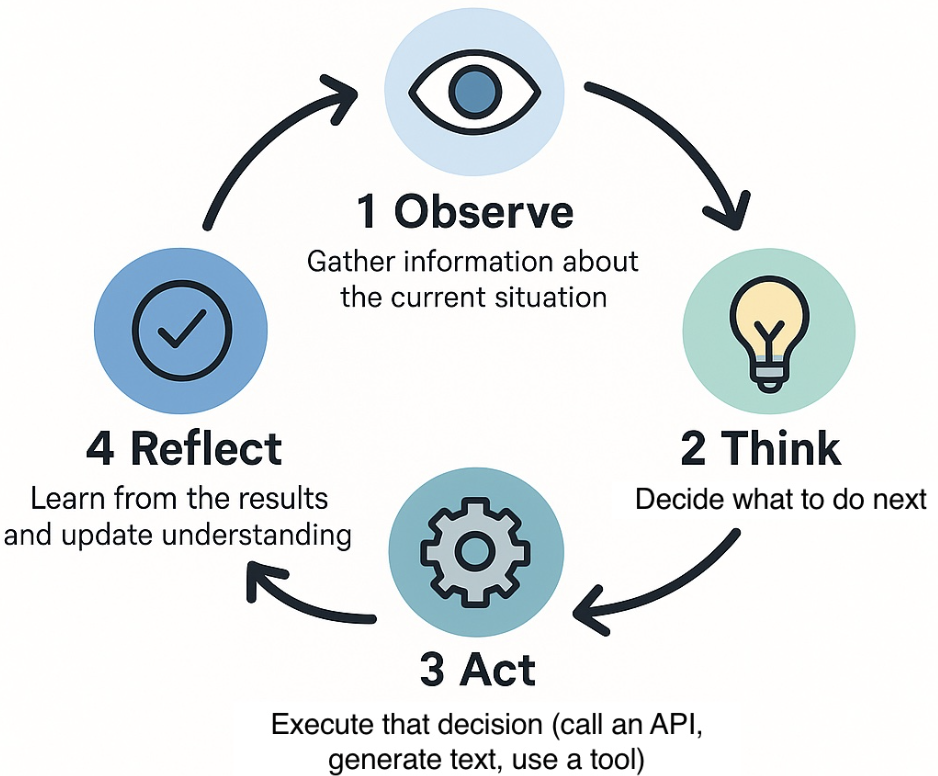
\includegraphics[width=0.58\linewidth,height=1.35in,keepaspectratio]{ailoop.png}
  \end{center}
\end{frame}

\begin{frame}[shrink=25]{Percepts, Percept Sequences, And The Environment}
  \begin{cpdefinition}
    A \textbf{percept} is what an agent senses at a particular moment. A \textbf{percept sequence} is the complete history of the agent's percepts.
  \end{cpdefinition}
  \vspace{0.10in}
  \begin{itemize}
    \item The current percept tells the agent what its sensors report \emph{now}.
    \item The percept sequence preserves what has happened over time.
    \item The relevant \textbf{environment} is not necessarily the whole universe; it is the part of the world that matters to the agent's task.
  \end{itemize}
  \vspace{0.10in}
  \begin{exampleblockcp}
    A vacuum robot's sequence might include: clean floor, dirt detected, wall ahead, turn left, low battery, charger detected.
  \end{exampleblockcp}
  \vspace{0.08in}
  \begin{keyidea}
    History matters whenever the same current percept can mean different things depending on what happened earlier.
  \end{keyidea}
\end{frame}

% ============================================================
\sectionframe{Part 2: Agent Functions And Programs}
% ============================================================

\begin{frame}{Vacuum Bot: What Choices Does It Make?}
  \begin{columns}[T,onlytextwidth]
    \begin{column}{0.48\textwidth}
      \lectureimage[2.0in]{vacuumbot.png}
    \end{column}
    \begin{column}{0.47\textwidth}
      \begin{itemize}
        \item Move forward, turn, or stop?
        \item Clean here or continue exploring?
        \item Avoid an obstacle or choose another route?
        \item Return to charge or keep working?
        \item Revisit an area or assume it is already clean?
      \end{itemize}
      \vspace{0.10in}
      \begin{activity}
        Which percepts should determine each choice?
      \end{activity}
    \end{column}
  \end{columns}
\end{frame}

\begin{frame}{Agent Function: The Abstract Model}
  \begin{columns}[T,onlytextwidth]
    \begin{column}{0.53\textwidth}
      \begin{cpdefinition}
        The \textbf{agent function} maps every possible percept sequence to an action.
      \end{cpdefinition}
      \vspace{0.10in}
      \begin{itemize}
        \item It is a theoretical, mathematical description of how an agent behaves.
        \item It specifies an action for every percept history the agent could encounter.
        \item Written literally as a table, it would be enormous and can be potentially infinite.
      \end{itemize}
      \vspace{0.08in}
      \begin{center}
        {\Large $f : P^* \rightarrow A$}
      \end{center}
    \end{column}
    \begin{column}{0.40\textwidth}
      \lectureimage[2.0in]{intelligentagents.png}
    \end{column}
  \end{columns}
\end{frame}

\begin{frame}[shrink=35]{Vacuum Cleaner Agent Function}
  \begin{columns}[T,onlytextwidth]
    \begin{column}{0.51\textwidth}
      \begin{keyidea}
        The abstract function must define an action for \emph{every possible percept sequence}, not merely for the current sensor reading.
      \end{keyidea}
      \vspace{0.08in}
      \begin{itemize}
        \item Percepts might include room location, dirt status, obstacles, and battery state.
        \item The history might include every room visited and every earlier sensor reading.
        \item Possible actions include moving, turning, cleaning, stopping, and docking.
      \end{itemize}
      \vspace{0.08in}
      \begin{exampleblockcp}
        The old vacuum-world table maps sequences such as $(A,\text{Dirty})$ or $(A,\text{Clean}),(B,\text{Dirty})$ to actions such as \texttt{Suck}, \texttt{Right}, or \texttt{Left}.
      \end{exampleblockcp}
    \end{column}
    \begin{column}{0.43\textwidth}
      \lectureimage[2.0in]{functiontable.png}
    \end{column}
  \end{columns}
\end{frame}

\begin{frame}[shrink=35]{Agent Program: The Concrete Implementation}
  \begin{columns}[T,onlytextwidth]
    \begin{column}{0.53\textwidth}
      \begin{cpdefinition}
        An \textbf{agent program} is the actual code or system that implements an agent function on a physical or software architecture.
      \end{cpdefinition}
      \vspace{0.08in}
      \begin{itemize}
        \item It runs on hardware and determines actions from percepts.
        \item It is \emph{not} the same thing as the abstract agent function; it is one practical way to approximate or implement that function.
        \item A real program generalizes behavior rather than storing every possible percept sequence explicitly.
      \end{itemize}
      \vspace{0.08in}
      \begin{exampleblockcp}
        Vacuum program: if dirt is detected, clean; else if an obstacle is detected, turn; otherwise move forward.
      \end{exampleblockcp}
    \end{column}
    \begin{column}{0.40\textwidth}
      \lectureimage[2.0in]{vacuumbotdecision.png}
    \end{column}
  \end{columns}
\end{frame}

% ============================================================
\sectionframe{Part 3: Rational Agents}
% ============================================================

\begin{frame}{Aristotle's Practical Reasoning}
  \begin{exampleblockcp}
    ``The function of man is an activity of the soul in accordance with reason.''
  \end{exampleblockcp}
  \vspace{0.08in}
  \begin{columns}[T,onlytextwidth]
    \begin{column}{0.46\textwidth}
      \begin{block}{Theoretical Reasoning}
        Knowing what is true.
      \end{block}
    \end{column}
    \begin{column}{0.46\textwidth}
      \begin{block}{Practical Reasoning}
        Deciding what to do in order to achieve a goal.
      \end{block}
    \end{column}
  \end{columns}
\end{frame}

\begin{frame}[shrink=10]{Vacuum Bot: Is It Rational?}
  \begin{columns}[T,onlytextwidth]
    \begin{column}{0.56\textwidth}
      \lectureimage[2.25in]{vacuumrational.png}
    \end{column}
    \begin{column}{0.38\textwidth}
      \begin{activity}
        Is a vacuum bot rational?
      \end{activity}
      \vspace{0.12in}
      \begin{activity}
        Are \emph{you} rational?
      \end{activity}
      \vspace{0.12in}
      \begin{keyidea}
        Rationality is not about being human, conscious, or always correct. It is about choosing actions well relative to information and objectives.
      \end{keyidea}
    \end{column}
  \end{columns}
\end{frame}

\begin{frame}{Rationality Versus Omniscience}
  \begin{columns}[T,onlytextwidth]
    \begin{column}{0.49\textwidth}
      \begin{block}{Omniscience --- Impossible}
        A truly omniscient agent would know the \emph{actual} outcome of every possible action before acting.
      \end{block}
      \begin{itemize}
        \item It would know the future.
        \item It could always select the action with the best realized outcome.
        \item Real agents do not have this information.
      \end{itemize}
    \end{column}
    \begin{column}{0.49\textwidth}
      \begin{block}{Rationality --- Possible}
        A rational agent chooses the action expected to maximize performance from the information available.
      \end{block}
      \begin{itemize}
        \item Success is probabilistic, not guaranteed.
        \item A rational decision may still fail.
        \item What matters is the quality of the decision given the evidence.
      \end{itemize}
    \end{column}
  \end{columns}
  \vspace{0.08in}
  \begin{center}
    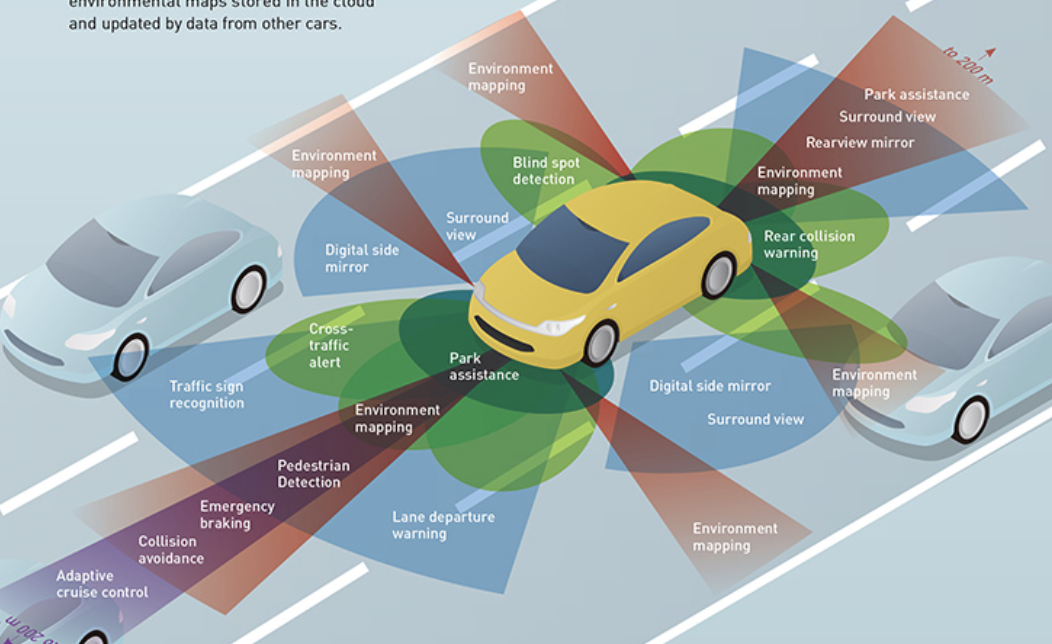
\includegraphics[width=0.58\linewidth,height=1.25in,keepaspectratio]{omniscient.png}
  \end{center}
\end{frame}

\begin{frame}[shrink=10]{Rationality Is Not Perfection}
  \begin{columns}[T,onlytextwidth]
    \begin{column}{0.52\textwidth}
      \begin{block}{Rationality}
        Act on available information to maximize expected success.
      \end{block}
      \begin{block}{Perfection}
        Always choose the action that turns out best---which would require advance knowledge of uncertain future events.
      \end{block}
      \vspace{0.08in}
      \begin{keyidea}
        AI does not need to be omniscient. It needs to be good enough at making decisions with limited knowledge.
      \end{keyidea}
    \end{column}
    \begin{column}{0.42\textwidth}
      \lectureimage[2.0in]{omniscient.png}
    \end{column}
  \end{columns}
\end{frame}

% ============================================================
\sectionframe{Part 4: Learning And Autonomy}
% ============================================================

\begin{frame}{Not Learning: The Danger Of Rigid Behavior}
  \begin{columns}[T,onlytextwidth]
    \begin{column}{0.56\textwidth}
      \begin{keyidea}
        Some agents do not need to learn if the world is perfectly predictable---but that makes them fragile.
      \end{keyidea}
      \vspace{0.12in}
      \begin{itemize}
        \item A fixed routine can be extremely effective in the environment it was designed for.
        \item A small change in the world can invalidate assumptions embedded in the routine.
        \item Without learning, the agent cannot improve from failure or adapt to new conditions.
      \end{itemize}
    \end{column}
    \begin{column}{0.36\textwidth}
      \lectureimage[2.1in]{ridgidbehavior.png}
    \end{column}
  \end{columns}
\end{frame}

\begin{frame}{Learning: Rational Agents Modify Future Percepts}
  \begin{columns}[T,onlytextwidth]
    \begin{column}{0.52\textwidth}
      \begin{itemize}
        \item Actions should sometimes be taken not only to achieve an immediate goal, but also to gather useful information.
        \item Example: looking both ways before crossing the street improves the quality of the next decision.
        \item A rational agent must balance \textbf{acting} with \textbf{exploring}.
      \end{itemize}
      \vspace{0.10in}
      \begin{exampleblockcp}
        An action can change the world, but it can also change what the agent will be able to perceive and learn next.
      \end{exampleblockcp}
    \end{column}
    \begin{column}{0.42\textwidth}
      \lectureimage[2.0in]{learning.png}
    \end{column}
  \end{columns}
\end{frame}

\begin{frame}[shrink=15]{Exploration In Unknown Environments}
  \begin{columns}[T,onlytextwidth]
    \begin{column}{0.52\textwidth}
      \begin{itemize}
        \item A vacuum bot placed in an unknown room may need to explore before it can clean efficiently.
        \item It must learn where obstacles, walls, open regions, and charging locations are.
        \item Rational agents adapt from new percepts rather than relying entirely on pre-programmed knowledge.
        \item Exploration creates information that can improve future performance.
      \end{itemize}
      \vspace{0.10in}
      \begin{keyidea}
        Exploration is useful because knowledge itself can have future value.
      \end{keyidea}
    \end{column}
    \begin{column}{0.42\textwidth}
      \lectureimage[2.0in]{exploration.png}
    \end{column}
  \end{columns}
\end{frame}

\begin{frame}{Alan Turing On Learning (1950)}
  \begin{columns}[T,onlytextwidth]
    \begin{column}{0.57\textwidth}
      \begin{exampleblockcp}
        ``Instead of trying to produce a programme to simulate the adult mind, why not rather try to produce one which simulates the child's?''
      \end{exampleblockcp}
      \vspace{0.10in}
      \begin{itemize}
        \item Turing suggested that intelligence need not be fixed at design time.
        \item Experience and environment can shape what a system becomes capable of doing.
        \item This aligns with the idea of agents that adapt rather than simply arriving ``smart.''
      \end{itemize}
    \end{column}
    \begin{column}{0.35\textwidth}
      \lectureimage[2.0in]{chappie.png}
    \end{column}
  \end{columns}
\end{frame}

\begin{frame}{Autonomy}
  \begin{columns}[T,onlytextwidth]
    \begin{column}{0.56\textwidth}
      \begin{cpdefinition}
        \textbf{Autonomy} is the degree to which an agent relies on its own percepts and learning rather than only on pre-programmed knowledge.
      \end{cpdefinition}
      \vspace{0.10in}
      \begin{itemize}
        \item An agent that only follows hard-coded rules has limited autonomy.
        \item Experience can allow an agent to compensate for gaps in its initial knowledge.
        \item A fully rational agent should be able to adapt and learn when the world differs from its initial assumptions.
      \end{itemize}
    \end{column}
    \begin{column}{0.38\textwidth}
      \lectureimage[2.0in]{autonomy.png}
    \end{column}
  \end{columns}
\end{frame}

\begin{frame}[shrink=15]{Autonomy: Prior Knowledge And Learning}
  \begin{columns}[T,onlytextwidth]
    \begin{column}{0.54\textwidth}
      \begin{block}{Balancing prior knowledge and learning}
        Total autonomy from the start is not practical. An agent with no prior knowledge would have no reason to prefer one initial action over another.
      \end{block}
      \begin{block}{The power of learning}
        With enough experience, an agent's behavior can become increasingly independent from its initial programming.
      \end{block}
      \begin{itemize}
        \item Learning lets one intelligent system succeed across a wider variety of environments.
        \item Built-in knowledge gives the agent a useful starting point; experience improves it.
      \end{itemize}
    \end{column}
    \begin{column}{0.39\textwidth}
      \lectureimage[2.0in]{autonomy.png}
    \end{column}
  \end{columns}
\end{frame}

% ============================================================
\sectionframe{Part 5: Task Environments And PEAS}
% ============================================================

\begin{frame}[shrink=20]{The Problem Agents Must Solve}
  \begin{columns}[T,onlytextwidth]
    \begin{column}{0.52\textwidth}
      \begin{keyidea}
        A \textbf{task environment} is the problem, and a rational agent is the proposed solution.
      \end{keyidea}
      \vspace{0.08in}
      \begin{itemize}
        \item Before designing an agent, we should define the environment in which it will operate.
        \item The \textbf{PEAS} framework forces us to specify the task clearly.
      \end{itemize}
      \vspace{0.06in}
      \begin{block}{PEAS}
        \textbf{P}erformance measure\\
        \textbf{E}nvironment\\
        \textbf{A}ctuators\\
        \textbf{S}ensors
      \end{block}
    \end{column}
    \begin{column}{0.42\textwidth}
      \lectureimage[2.0in]{taxi.png}
    \end{column}
  \end{columns}
\end{frame}

\begin{frame}{PEAS Example: Self-Driving Taxi}
  \begin{columns}[T,onlytextwidth]
    \begin{column}{0.23\textwidth}
      \begin{block}{Performance}
        Safety, passenger comfort, trip efficiency, obeying traffic laws, maximizing profits.
      \end{block}
    \end{column}
    \begin{column}{0.23\textwidth}
      \begin{block}{Environment}
        Roads, traffic, pedestrians, weather, passengers, obstacles.
      \end{block}
    \end{column}
    \begin{column}{0.23\textwidth}
      \begin{block}{Actuators}
        Steering, acceleration, braking, signals, doors.
      \end{block}
    \end{column}
    \begin{column}{0.23\textwidth}
      \begin{block}{Sensors}
        Cameras, lidar, GPS, speedometer, proximity sensors.
      \end{block}
    \end{column}
  \end{columns}
  \vspace{0.10in}
  \begin{keyidea}
    PEAS is not an implementation. It is a disciplined specification of what the agent is supposed to accomplish and what information and actions are available.
  \end{keyidea}
\end{frame}

\begin{frame}{PEAS Examples}
  \scriptsize
  \begin{center}
  \resizebox{\linewidth}{!}{%
    \begin{tabular}{|l|p{2.7cm}|p{3.0cm}|p{2.8cm}|p{3.0cm}|}
      \hline
      \textbf{Agent Type} & \textbf{Performance Measure} & \textbf{Environment} & \textbf{Actuators} & \textbf{Sensors} \\
      \hline
      Water bottle fill station & Actually turns ON/OFF & Students, water bottles & Water valve & Proximity sensor \\
      \hline
      Grubhub delivery robot & On-time delivery, minimal spillage & Campus pathways, pedestrians, traffic & Wheels, delivery compartment door & GPS, cameras, lidar, proximity sensors \\
      \hline
      Code autograder & Accurate scoring, fair feedback & Student code submissions & Display of grades, feedback messages & Code input, test-case results \\
      \hline
      AC thermostat & Comfort, energy efficiency & A room or building & Heater/cooler switches, fan control & Temperature sensor, humidity sensor \\
      \hline
      Part-picking robot & Percentage of parts in correct bins & Conveyor belt with parts, bins & Jointed arm, gripper & Camera, tactile sensors, joint-angle sensors \\
      \hline
    \end{tabular}}
  \end{center}
  \vspace{0.08in}
  \begin{center}
    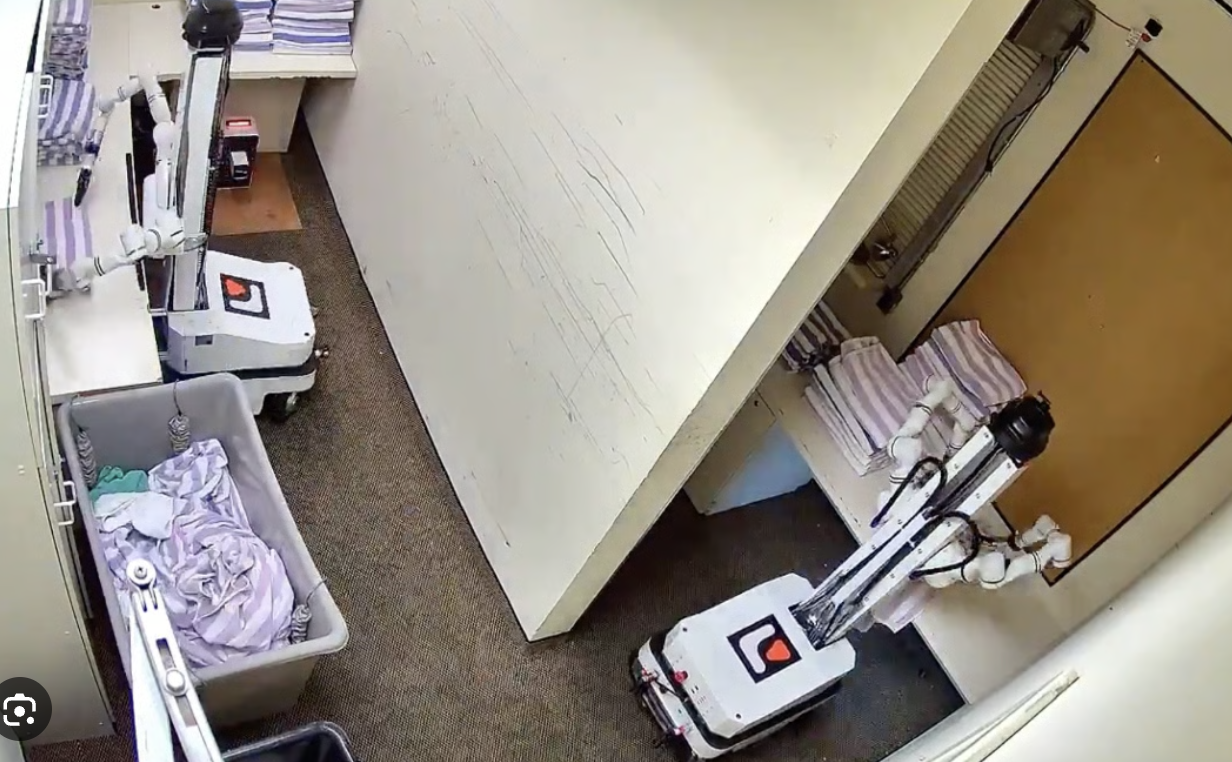
\includegraphics[width=0.46\linewidth,height=1.05in,keepaspectratio]{foldingroboto.png}
  \end{center}
\end{frame}

% ============================================================
\sectionframe{Part 6: Properties Of Task Environments}
% ============================================================

\begin{frame}{Observability: How Much Can The Agent See?}
  \begin{columns}[T,onlytextwidth]
    \begin{column}{0.31\textwidth}
      \begin{block}{Fully Observable}
        The agent has complete information about the relevant environment state at all times.
      \end{block}
      \begin{exampleblockcp}
        Chess: every piece is visible on the board.
      \end{exampleblockcp}
    \end{column}
    \begin{column}{0.31\textwidth}
      \begin{block}{Partially Observable}
        The agent receives limited, noisy, or incomplete information.
      \end{block}
      \begin{exampleblockcp}
        Self-driving car: sensors cannot see around every corner.
      \end{exampleblockcp}
    \end{column}
    \begin{column}{0.31\textwidth}
      \begin{block}{Unobservable}
        The agent has no direct perceptual access to the relevant environment state.
      \end{block}
      \begin{exampleblockcp}
        A robot attempting to navigate with no usable sensing.
      \end{exampleblockcp}
    \end{column}
  \end{columns}
\end{frame}

\begin{frame}{Single-Agent Versus Multi-Agent}
  \begin{columns}[T,onlytextwidth]
    \begin{column}{0.47\textwidth}
      \begin{block}{Single-Agent}
        The agent operates alone; other decision-making agents do not significantly affect the task.
      \end{block}
      \begin{exampleblockcp}
        Vacuum cleaner in an empty house.
      \end{exampleblockcp}
    \end{column}
    \begin{column}{0.47\textwidth}
      \begin{block}{Multi-Agent}
        Other agents exist and their choices influence the environment.
      \end{block}
      \begin{exampleblockcp}
        A swarm of delivery drones, traffic, games, or markets.
      \end{exampleblockcp}
    \end{column}
  \end{columns}
  \vspace{0.08in}
  \begin{columns}[T,onlytextwidth]
    \begin{column}{0.47\textwidth}
      \begin{block}{Competitive}
        Agents work against one another, as in chess or trading.
      \end{block}
    \end{column}
    \begin{column}{0.47\textwidth}
      \begin{block}{Cooperative}
        Agents coordinate toward shared objectives, as in robot teams.
      \end{block}
    \end{column}
  \end{columns}
\end{frame}

\begin{frame}{Deterministic Versus Stochastic}
  \begin{columns}[T,onlytextwidth]
    \begin{column}{0.47\textwidth}
      \begin{block}{Deterministic}
        The next state is fully determined by the current state and the agent's action.
      \end{block}
      \begin{exampleblockcp}
        Sliding puzzle: under the model, moving a tile has a definite result.
      \end{exampleblockcp}
    \end{column}
    \begin{column}{0.47\textwidth}
      \begin{block}{Stochastic / Nondeterministic}
        Outcomes are uncertain; the same state and action can lead to different results.
      \end{block}
      \begin{exampleblockcp}
        Poker: hidden cards and uncertain opponent behavior affect outcomes.
      \end{exampleblockcp}
    \end{column}
  \end{columns}
\end{frame}

\begin{frame}{Episodic Versus Sequential}
  \begin{columns}[T,onlytextwidth]
    \begin{column}{0.47\textwidth}
      \begin{block}{Episodic}
        Each decision is independent; earlier actions do not affect later decisions.
      \end{block}
      \begin{exampleblockcp}
        Image classification: each image can be analyzed separately.
      \end{exampleblockcp}
    \end{column}
    \begin{column}{0.47\textwidth}
      \begin{block}{Sequential}
        Future decisions depend on previous actions and the states they created.
      \end{block}
      \begin{exampleblockcp}
        Video tracking, driving, games, and navigation.
      \end{exampleblockcp}
    \end{column}
  \end{columns}
\end{frame}

\begin{frame}{Static Versus Dynamic}
  \begin{columns}[T,onlytextwidth]
    \begin{column}{0.47\textwidth}
      \begin{block}{Static}
        The environment does not change while the agent deliberates unless an agent acts.
      \end{block}
      \begin{exampleblockcp}
        Chess without a clock: the board does not change on its own.
      \end{exampleblockcp}
    \end{column}
    \begin{column}{0.47\textwidth}
      \begin{block}{Dynamic}
        The world can change while the agent is deciding.
      \end{block}
      \begin{exampleblockcp}
        Self-driving car: traffic continues moving while the car plans.
      \end{exampleblockcp}
    \end{column}
  \end{columns}
\end{frame}

\begin{frame}{Discrete Versus Continuous}
  \begin{columns}[T,onlytextwidth]
    \begin{column}{0.47\textwidth}
      \begin{block}{Discrete}
        The relevant states, percepts, actions, or time steps form a finite or countable set.
      \end{block}
      \begin{exampleblockcp}
        Chess: legal moves are discrete alternatives.
      \end{exampleblockcp}
    \end{column}
    \begin{column}{0.47\textwidth}
      \begin{block}{Continuous}
        States or actions vary over continuous ranges.
      \end{block}
      \begin{exampleblockcp}
        A robotic arm can vary joint positions and velocities continuously.
      \end{exampleblockcp}
    \end{column}
  \end{columns}
\end{frame}

\begin{frame}{Known Versus Unknown}
  \begin{columns}[T,onlytextwidth]
    \begin{column}{0.47\textwidth}
      \begin{block}{Known}
        The agent understands the rules that determine how actions affect the environment.
      \end{block}
      \begin{exampleblockcp}
        Chess AI: legal moves and game rules are known.
      \end{exampleblockcp}
    \end{column}
    \begin{column}{0.47\textwidth}
      \begin{block}{Unknown}
        The agent must learn how the world works through experience.
      \end{block}
      \begin{exampleblockcp}
        A newly built robot exploring unfamiliar terrain while localizing itself.
      \end{exampleblockcp}
    \end{column}
  \end{columns}
\end{frame}

\begin{frame}{Environments?}
  \scriptsize
  \begin{center}
  \resizebox{\linewidth}{!}{%
    \begin{tabular}{|l|c|c|c|c|c|c|}
      \hline
      \textbf{Task Environment} & \textbf{Observable} & \textbf{Agents} & \textbf{Deterministic} & \textbf{Episodic} & \textbf{Static} & \textbf{Discrete} \\
      \hline
      Crossword puzzle & Fully & Single & Deterministic & Sequential & Static & Discrete \\
      Chess with a clock & Fully & Multi & Deterministic & Sequential & Semi & Discrete \\
      \hline
      Poker & Partially & Multi & Stochastic & Sequential & Static & Discrete \\
      Backgammon & Fully & Multi & Stochastic & Sequential & Static & Discrete \\
      \hline
      Taxi driving & Partially & Multi & Stochastic & Sequential & Dynamic & Continuous \\
      Medical diagnosis & Partially & Single & Stochastic & Sequential & Dynamic & Continuous \\
      \hline
      Image analysis & Fully & Single & Deterministic & Episodic & Semi & Continuous \\
      Part-picking robot & Partially & Single & Stochastic & Episodic & Dynamic & Continuous \\
      \hline
      Refinery controller & Partially & Single & Stochastic & Sequential & Dynamic & Continuous \\
      English tutor & Partially & Multi & Stochastic & Sequential & Dynamic & Discrete \\
      \hline
    \end{tabular}}
  \end{center}
  \vspace{0.08in}
  \begin{keyidea}
    These labels are modeling assumptions. A task can move between categories when we change what counts as the state, what sensors are available, or what uncertainty we include.
  \end{keyidea}
\end{frame}

\end{document}
